\documentclass[
	twoside,
%	draft,
	fontsize=12pt,
	headsepline,
	cleardoublepage=empty,
	numbers=noenddot,
%	bibliography=totoc,
]{scrbook}

\usepackage{ks}
\usepackage{subfigure}

% customize name, title, ...
\renewcommand{\thesisAuthor}{Julian Daberkow\\Julian Exner\\Andreas Gatting\\Timo Michalski\\Hendrik Oestreich}
\renewcommand{\thesisStudNum}{1234567}
\renewcommand{\thesisTitle}{Autonomes Ladeverhalten für den AMiRo\\im Rahmen eines Fußballszenarios }
\renewcommand{\thesisDate}{Bielefeld, März 2016}
\renewcommand{\thesisId}{}
\renewcommand{\thesisType}{Projektbericht}
\renewcommand{\thesisCourse}{Autonomous Systems Engineering}
\renewcommand{\thesisSupervisor}{M.Sc.~Timo~Korthals\\M.Sc.~Thomas~Schöpping}

\makeatletter
\newcommand{\sectionauthor}[1]{%
	{\vspace{-35pt}\hfill\scshape#1}\\
	\@afterheading%
}
\makeatother

% hyphenation
\hyphenation{
Pro-zes-sor-e-le-men-te
Pro-zes-sor-e-le-men-ten
Pro-zes-sor-e-le-men-tes
}
\graphicspath{ {media/} }
\begin{document}
\pagenumbering{roman}
\begin{titlepage}
\fontfamily{phv}
\fontseries{m}
\selectfont
\leftskip2em

\begin{minipage}[t]{0.4\textwidth}
\large \thesisType\\
\normalsize \thesisCourse
\end{minipage}
\hfill
\begin{minipage}[t]{0.4\textwidth}
\begin{flushright}
CITEC, Universität Bielefeld\\
AG Kognitronik \& Sensorik \\
Prof. Dr.-Ing. Ulrich Rückert     
\end{flushright}
\end{minipage}

\vfill

{\fontfamily{phv}\fontseries{bc}\selectfont 
\Huge \thesisTitle
\begin{flushright}
\Large \thesisAuthor
\end{flushright}
}

\vfill

\normalsize
%\begin{minipage}[t]{5em}
%Matr.-Nr.:\quad
%\end{minipage}
%\begin{minipage}[t]{0.5\textwidth}
%\thesisStudNum
%\end{minipage}

\begin{minipage}[t]{5em}
Betreuer:\quad
\end{minipage}
\begin{minipage}[t]{0.5\textwidth}
\thesisSupervisor
\end{minipage}




\vfill

\thesisDate
\hfill
\thesisId

% enlarge page by 2 lines
\enlargethispage{2\baselineskip}

\end{titlepage}

\cleardoublepage
\subsection*{Kurzfassung}

Um autonome Paradigmen für Miniroboter in einem größeren Zeitfenster etablieren zu können, wird eine autark bewerkstelligte Energieversorgung benötigt. In der vereinfachten Welt des Schaukastens wurden in diesem Projekt dafür die Lokalisation der Ladestation, das Anfahren und Einparken sowie das Andocken an den Lademechanismus realisiert. Zur Einbettung in einen anwendungsorientieren Kontext wurde zudem ein Fußballszenario implementiert, in dem zwei AMiRos gegeneinander antreten. Dabei wird das Szenario extern überwacht und spielentscheidende Elemente werden identifiziert und visualisiert. 


\tableofcontents

%% content
\cleardoublepage
\pagenumbering{arabic}

\chapter[Einleitung]{Einleitung \hfill\raggedleft{\normalsize J.D.}} \label{kap:einleitung} %TODO: Julian D.
- Bezug nehmen auf Vorlesungsinhalte --> Übertragung auf realisiertes Projekt

- Ziele und Voraussetzungen einarbeiten:\\
Ziele:\\
Fußball Tipp-Kick Szenario \\
Autonome Ladestrategien für AMiRos\\
Spieltracking durch Bildverarbeitung\\
\\
Voraussetzungen:\\
2 AMiRos\\
1 Ladestation\\
1 Schaukasten\\
1 Webcam\\
1 Host-PC\\
1 Router\\
2 Tore\\
1 Spielball\\
diverse AR-Marker\\

%TODO: 
Beschreibung der Kapitelautoren?
z.B. Hendrik Oestreich = H.O.
\chapter{Autonomes Ladeverhalten} \label{kap:AutonomesLadeverhalten}

\section[Lokalisation der Ladestation]{Lokalisation der Ladestation\hfill {\normalsize A.G.}} %TODO: Andi G.

\section[Finite-State-Machine des DiWheelDrive-Microcontrollers]{Finite-State-Machine des DiWheelDrive-Microcontrollers\hfill {\normalsize J.E. \& T.M.}} %TODO: Julian E. & Timo M.

Nachdem die Ladestation erfolgreich angefahren wurde, wird durch eine CAN-Nachricht dem DiWheelDrive-Board signalisiert, dass die weiteren Schritte des Einparkens eingeleitet werden sollen.
Auf dem Microcontroller wird eine State-Machine ausgeführt, die so lange im \textit{IDLE}-Zustand wartet, bis das Ladeverhalten angetriggert wird (siehe Abb. \ref{fig:uC_statmachine}).
Der nächste Zustand ist \textit{MOVE INTO STATION}, welcher in Kapitel \ref{kap:einparken_ladestation} erläutert wird. Ist dies erfolgreich abgeschlossen, so folgen die Zustände \textit{TURN AROUND} und \textit{ADJUST POSITION}, welche in Kapitel \ref{kap:andocken_ladestation} erklärt werden. Anschließend wird der Ladevorgang des AMiRos gestartet und überwacht. Dies geschieht in den Zuständen \textit{INITIATE CHARGING} und \textit{CHARGING}. Diese sind im Kapitel \ref{kap:ladevorgang} beschrieben.

Sollte ein Zustand nicht erfolgreich ausgeführt werden können, so gibt es definierte Routinen, die abermals ausgeführt werden müssen. Sollte die CAN-Nachricht für einen Abbruch des Ladevorganges eingehen, so wird dieser sofort unterbrochen und die State-Machine wird in den \textit{IDLE}-Zustand versetzt.

\begin{figure}[H]
	\begin{center}
		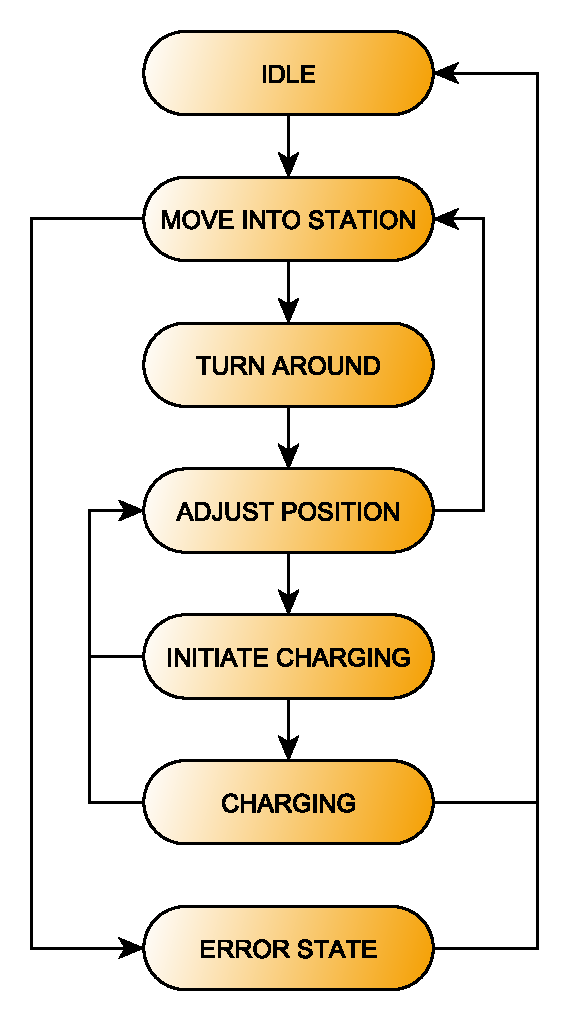
\includegraphics[width=0.4\textwidth]{uC_statemachine.pdf} 	
		\caption{Finite-State-Machine des DiWheelDrive-Microcontrollers}
		\label{fig:uC_statmachine}
	\end{center}
\end{figure}

\section[Einparken in der Ladestation]{Einparken in der Ladestation\hfill {\normalsize J.E.}}\label{kap:einparken_ladestation} %TODO: Julian E.

\section[Andocken an die Ladestation]{Andocken an die Ladestation\hfill {\normalsize T.M.}}\label{kap:andocken_ladestation} %TODO: Timo M.
Nachdem der AMiRo erfolgreich in der Ladestation eingeparkt ist werden anschließend die Ladepins auf der Rückseite des Roboters zu den Ladekontakten der Station ausgerichtet. Dabei ist es notwendig, dass alle Pins die Kontakte berühren, da es bei Stromspitzen sonst zu Schäden am AMiRo kommen könnte.

Als ersten Schritt wird zunächst eine 180$^\circ$ Drehung durchgeführt, durch die der AMiRo grob in die Ladeposition gedreht wird. Die Drehung wird anhand der Odometriedaten des Roboters durchgeführt. Dabei kann eine gewünschte Fehlertoleranz als Argument übergeben werden. Da eine exakte Drehung um 180$^\circ$ kompliziert ist, wird hier eine Fehlertoleranz von 5$^\circ$ eingeräumt, damit die Drehung schnell durchgeführt werden kann und der AMiRo nicht die Position mehrfach verbessern muss, bis exakt 180$^\circ$ erreicht sind. Diese Toleranz hat auf das anschließende Justieren der Position keine Auswirkungen.

Für die Justierung der Ladeposition des AMiRos werden die Daten der beiden hinteren Abstandssensoren genutzt. Um diese zur Ausrichtung des Roboters nutzen zu können, wurden an der Station zwei schwarze Streifen angebracht (siehe Abb. \ref{fig:charging_station}). Diese bieten einen hohen Kontrast für die UV-Sensoren im Vergleich zur weißen Station. So liefern die Sensoren den maximalen Wert von 0xFFFF, wenn sie sich direkt vor der weißen Ladestation befinden und einen im Vergleich sehr niedrigen Wert von unter 0x2000, wenn sie den Abstand zu einen schwarzen Klebestreifen messen. 
Die Klebestreifen sind so angebracht, dass sich beide hinteren Abstandssensoren genau vor einer weißen Fläche befinden, wenn die Ladeposition erreicht ist. 
Das heißt, dass die Position des AMiRos so lange justiert werden muss, bis beide Sensoren den Wert 0xFFFF liefern. 
Dafür werden die Werte der Abstandssensoren ausgelesen und anhand dieser wird nun unterschieden in welcher Position sich der AMiRo befindet und welches der nächste Schritt ist, um die Ladeposition zu erreichen. 

\begin{figure}[]
	\begin{center}
		\includegraphics[width=0.6\textwidth]{charging_station_stripes.jpg} 	
		\caption{Ladestation mit Klebestreifen}
		\label{fig:charging_station}
	\end{center}
\end{figure}

Sollte einer der beiden Sensoren 0xFFFF als Wert liefern und der andere einen zu 0xFFFF abweichenden Wert, so steht der AMiRo direkt vor der Wand der Station, muss aber noch in die Richtung des Sensors mit vollem Ausschlag gedreht werden. Da der Magnet der Station eine hohe Anziehung auf die hintere Befestigungsschraube des AMiRos ausübt, ist es nicht möglich den Roboter durch minimales Ansteuern der PWM\footnote{Pulsweitenmodulation}-Steuerung der Motoren zu drehen. Deshalb fährt der Roboter ein kleines Stück aus der Station heraus um sich anschließend in die gegebene Richtung in die Station hinein zu bewegen. 
Wenn ein Sensor einen Wert über 0x4000 und der andere unter 0x4000 liefert, bedeutet dies, dass sich der AMiRo mit einem Abstand vor der Station befindet und seine Position außerdem ein wenig verdreht ist. In dieser Situation muss sich der Roboter in die Richtung des Sensors mit höherem Wert drehen und sich auf die Station zu bewegen. 
Geben beide Sensoren einen Wert über 0x4000 aus, so steht der AMiRo mit Abstand zur Station, muss jedoch nicht gedreht werden. In diesem Fall wird eine gerade Bewegung in Richtung der Station ausgeführt. 
Sollten beiden Sensoren einen Wert unter 0x4000 liefern, so steht der AMiRo in einem zu hohen Abstand zur Ladestation und das Einparken in die Ladestation wird nochmals eingeleitet.

Bevor der Ladevorgang eingeleitet wird, wird die Position des AMiRos nochmals überprüft. Hierfür werden die aktuellen Odometriedaten des Roboters abgerufen und gespeichert. Anschließend wird die PWM-Steuerung der Motoren deaktiviert, was zur Folge hat, dass sich die Reifen frei drehen können. Sollte der AMiRo noch nicht korrekt zur Ladestation ausgerichtet sein, kann die Position des Roboters durch die Wirkung des Magneten auf die Befestigungsschraube verändert werden. Dabei werden die aktuellen Odometriewerte mit den gespeicherten abgeglichen. Sollte sich nach einer Sekunde keine Änderung der Position ergeben haben, so wird eine korrekte Ladeposition angenommen und der Ladevorgang gestartet. Sollte sich die Odometrie verändern, so wird das Justieren nochmals eingeleitet. 




%- Ausgangssituation: AMiRo steht vorwärts in der Ladestation
%- 180$^\circ$ Drehung anhand der Odometrie um die Ladepins zur Station zu richten
%- Justierung der Position anhand der Abstandssensoren und der schwarzen Streifen
%- Abschalten der PWM und Überwachung, ob sich die Position ändert 
%	- Mögliche Fehlerquellen für Positionsänderung: 
%		- AMiRo wird durch den Einfluss des Magnetfeldes auf die Schraube gedreht, da die Position noch nicht gut genug justiert ist
%		- AMiRo wird durch die Federung der Ladepins von der Station abgestoßen, da die Schraube nicht genau vor dem Magneten war und somit die magnetische Kraft nicht groß genug war 

\section[Ansteuern und Überwachen des Ladevorgangs]{Ansteuern und Überwachen des Ladevorgangs\hfill {\normalsize T.M.}}\label{kap:ladevorgang} %TODO: Timo M.

Sobald der AMiRo mit seinen Ladepins zu den Ladekontakten der Ladestation ausgerichtet ist, kann der Ladevorgang eingeleitet werden.
Zunächst wird dem PowerManagement-Board signalisiert, dass der DiWheelDrive-Ladepfad aktiviert werden soll. Nun wird kontrolliert, ob wirklich mindestens 9V an den Pins anliegen und die Akkus aufgeladen werden. Hierfür wird eine kurze Zeit gewartet, da es aufgrund von Signalfilterungen bei der Ermittlung der anliegenden Spannung zu Verzögerungen kommt. Sollten anschließend keine 9V anliegen und die Akkus nicht geladen werden, so wird der Ladevorgang abgebrochen und die Position des AMiRos zur Station wird nochmals justiert.
Liegt die Spannung an und die Akkus werden geladen, so wird während des Ladevorgangs der Status mittels LEDs visualisiert (siehe Abb. \ref{fig:amiro_charging}). 
Währenddessen wird außerdem auf die Odometriedaten des AMiRos geachtet, denn sollte sich etwas an der Position des Roboters ändern, ist nicht mehr sichergestellt, dass alle Pins die Ladekontakte berühren und der Ladevorgang wird abgebrochen. Ein Grund hierfür könnten äußere Einwirkungen wie ein Wackeln am Schaukasten sein.

Nachdem die Akkus des AMiRos voll geladen sind wird der DiWheelDrive-Ladepfad deaktiviert, die PWM-Steuerung aktiviert und der Roboter fährt ein Stück aus der Ladestation heraus.

\begin{figure}[]
	\begin{center}
		\includegraphics[width=0.5\textwidth]{AMiRo_charging.jpg} 	
		\caption{Ladeanimation}
		\label{fig:amiro_charging}
	\end{center}
\end{figure}



%- Aktivieren des DiWheelDrive-Board Ladepfades (+ kurzes Abwarten)
%- Kontrolle, ob mehr als 9V anliegen (wenn nicht -> Position erneut justieren)
%- Überwachen des Ladevorgangs
%	- Auslesen der Ladestatus der Akkus (\% und Zeit bis geladen)
%	- Überwachen der Odometrie 
%		- falls sich der AMiRo aufgrund von äußeren Einwirkungen bewegen sollte -> Abbruch des Ladevorgangs und Position erneut justieren


\chapter{Fussballszenario} \label{kap:Fussballszenario} %TODO: Besseren Kapiteltitel

\section{Szenario Koordination} %TODO: Hendrik

\subsection{Kommunikation per RSB und Spread} %TODO: Hendrik

\subsection{Finite-State-Machine} %TODO: Hendrik

\begin{figure}[H]
	\begin{center}
		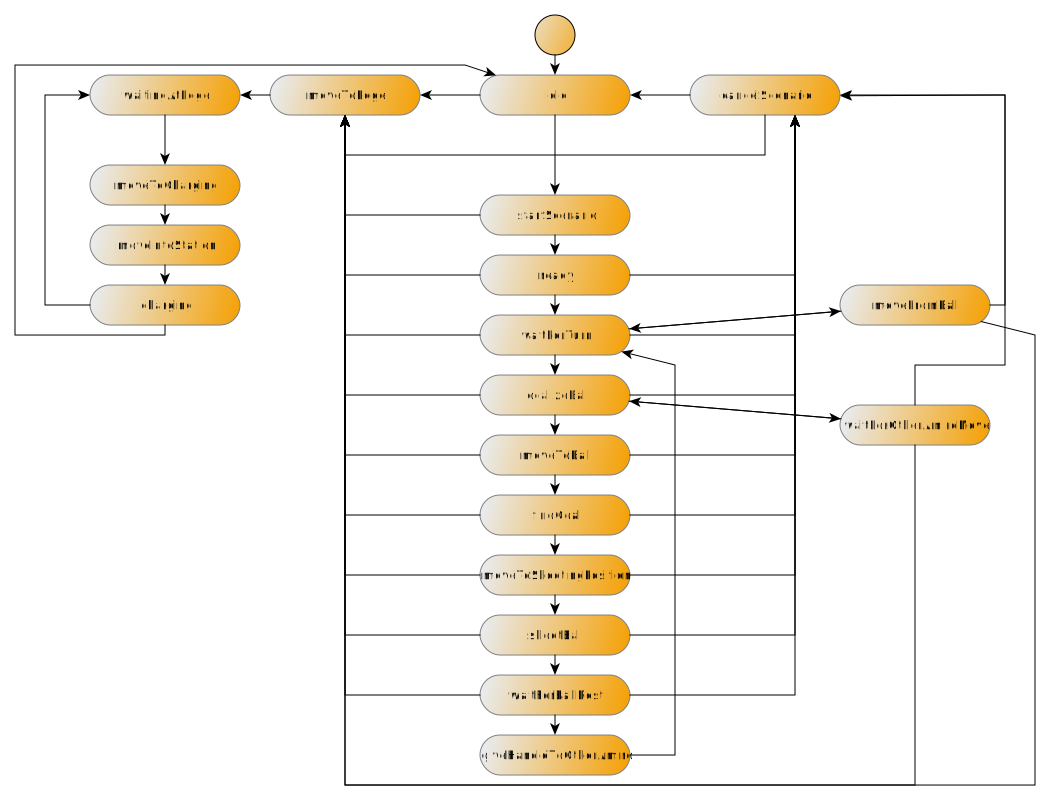
\includegraphics[scale=.55]{Final_FSM_AMiRo.pdf} 	
		\caption{Finite-State-Machine}
		\label{fig:fsm-amiro}
	\end{center}
\end{figure}

\section{Realisierung der einzelnen Spielelemente} %TODO: Besseren Sectiontitel

\subsection{Lokalisation des Balls} %TODO: Julian E.

\subsection{Anfahren des Balls} %TODO: Julian E.

\subsection{Lokalisation des gegnerischen Tores} %TODO: Timo M.

\subsection{Schussposition anfahren} %TODO: Timo M.

\subsection{Schießen} %TODO: Timo M.

\subsection{Beiseite Fahren} %TODO: Julian E. (Besseren Titel suchen^^)

\section{Spieltracking} %TODO: Julian D.

\subsection{Spielfeldbestimmung mit dem AR Toolkit} %TODO: Julian D.

\subsection{Extraktion wichtiger Spielelemente mit Bildverarbeitungsmethoden} %TODO: Julian D.

\subsection{Benutzerinteraktion mit AR Markern} %TODO: Julian D.

\subsection{Spielkoordination} %TODO: Julian D.

\subsection{Grafische Darstellung der Spielstatus} %TODO: Julian D.

% ...

\appendix
\listoffigures
%\lstlistoflistings
%\cleardoublepage
%\addcontentsline{toc}{chapter}{Literaturverzeichnis}
%\bibliographystyle{alpha}
%\bibliographystyle{geralpha} % benoetigt packet bibgerm
%\bibliography{literatur}
%\printbibliography

\chapter{Anhang}

\section{Spread Konfiguration}
\label{sec:spread-config}

AMiRo Kommunikation mit anderen AMiRos / Host:\\
(File=spreadShowcase.conf)

\lstset{language=bash}
\begin{lstlisting}
Spread_Segment  10.0.0.255:4803 {
	# amiro27
	stick1          10.0.0.201
}

Spread_Segment 10.0.0.255:4803 {
	# amiro23    
	stick0          10.0.0.202
}

Spread_Segment  10.0.0.255:4803 {
	lagomera        10.0.0.200
}
\end{lstlisting}

Interprozesskommunikation AMiRo:\\
(File=spreadShowcaseAMiRoInternal.conf)

\begin{lstlisting}
Spread_Segment  127.0.0.255:4806 {
	localhost               127.0.0.1
}
\end{lstlisting}


\section{RSB Konfiguration}
\label{sec:rsb-config}
AMiRo RSB Konfiguration\\
(File=rsb.conf)

\begin{lstlisting}
[plugins.cpp]
load = rsbspread
[transport.inprocess]
enabled = 0
[transport.socket]
enabled = 0
[transport.spread]
enabled = 1
host = 127.0.0.1
port    = 4806
\end{lstlisting}


\section{W-LAN Konfiguration}
\label{sec:wlan-config}
ASUS Router Konfiguration:\\
SSID: aseshowcase\\
PASS: aseshowcase\\

IP Adressen:\\
lagomera 10.0.0.200\\
stick1 10.0.0.201\\
stick0 10.0.0.202\\

Allgemeine Konfiguration des Connman Netzwerkmanagers:\\
/var/lib/connman/<SSID>-psk.config
\begin{lstlisting}
[service_wifi_<hash>_managed_psk]
Type = wifi
Name = <SSID>
Passphrase = <passphrase>
\end{lstlisting}

Spezifische Konfigurationen der beiden AMiRos:\\
/var/lib/connman/aseshowcase-psk.config

stick1:
\begin{lstlisting}
[service_wifi_wifi_74da380645e3_
61736573686f77636173655f3547_managed_psk]
Type = wifi
Name = aseshowcase
Passphrase = aseshowcase
Hidden = false
IPv4 = dhcp
IPv6 = off
\end{lstlisting}

stick0:
\begin{lstlisting}
[service_wifi_wifi_74da380645f6_
61736573686f77636173655f3547_managed_psk]
Type = wifi
Name = aseshowcase
Passphrase = aseshowcase
Hidden = false
IPv4 = dhcp
IPv6 = off
\end{lstlisting}



%%
%\cleardoublepage
%\thispagestyle{empty}
%\subsection*{Erklärung}
%Ich versichere, dass ich die vorliegende wissenschaftliche Arbeit 
%selbstständig verfasst und keine anderen als die angegebenen
%Hilfsmittel verwendet habe. Die Stellen der Arbeit, die anderen 
%Werken dem Wortlaut oder dem Sinn nach entnommen sind, wurden 
%unter Angabe der Quelle als Entlehnung deutlich gemacht. Das 
%Gleiche gilt auch für beigegebene Skizzen und Darstellungen. Diese 
%Arbeit hat in gleicher oder ähnlicher Form meines Wissens nach 
%noch keiner Prüfungsbehörde vorgelegen.
%
%\thesisDate
%
%~
%
%~
%
%\thesisAuthor

\begin{thebibliography}{9}
	\bibitem[Brooks86]{Brooks:1986}
	Rodney A. Brooks, IEEE Journal Of Robotics And Automation, Volume RA-2 No.1 (March 1986).
	\newblock A Robust Layered Control System For A Mobile Robot
	
	\bibitem[Sicil07]{Siciliano:2007}
	Bruno Siciliano and Oussama Khatib. 2007. Chapter 8.3.1, Springer-Verlag New York, Inc., Secaucus, NJ, USA.
	\newblock Springer Handbook of Robotics
	
	
\end{thebibliography}
\end{document}

